% Replace these questions and solutions with your own homework.
\section*{Assignment notes}
This example demonstrates questions, solutions, equations, tables, figures,
and citations. Both entry points support mixed text, for example:
中文与 English 可以出现在同一段落中。

\problem{Concepts and citations}
Explain the benefits of structured typesetting and cite relevant sources.
\begin{solution}
Structured typesetting separates content from presentation and keeps headings,
equation numbers, and cross-references consistent. See the introduction to
\LaTeX{} in \citep{lamport1994} and the Chinese-language guide in \citep{liu2013}.
Multiple sources can be cited together \citep{lamport1994,knuth1984}.
The reference list is generated from \texttt{references.bib}; only cited entries
are included.
\end{solution}

\problem{Mathematical derivation}
\label{sec:mean}
Given $n$ observations $x_1,\ldots,x_n$, find the constant $a$ that minimizes
the sum of squared errors.
\begin{solution}
The objective and its first derivative are
\begin{align}
  L(a) &= \sum_{i=1}^{n}(x_i-a)^2, \\
  \frac{\mathrm{d}L}{\mathrm{d}a} &= -2\sum_{i=1}^{n}(x_i-a)=0.
\end{align}
The optimum is therefore the sample mean:
\begin{equation}
  a^*=\bar{x}=\frac{1}{n}\sum_{i=1}^{n}x_i.
  \label{eq:mean}
\end{equation}
Since $L''(a)=2n>0$ for $n\geq1$, this is the unique minimum.
\end{solution}

\clearpage % Start the results example on a fresh page; remove if not needed.
\problem{Results and discussion}
Apply the result from Question~\ref{sec:mean} to example data and discuss a limitation.
\begin{solution}
Equation~\eqref{eq:mean} gives the results in Table~\ref{tab:results}.

\begin{table}[htbp]
  \centering
  \caption{Example data and calculated means}
  \label{tab:results}
  \begin{tabular}{lrr}
    \toprule
    Data set & Sample size $n$ & Mean $\bar{x}$ \\
    \midrule
    A: $2,4,6$ & 3 & 4.0 \\
    B: $1,3,5,7$ & 4 & 4.0 \\
    \bottomrule
  \end{tabular}
\end{table}

\begin{figure}[htbp]
  \centering
  % An actual PNG image with illustrative data only; replace with your own.
  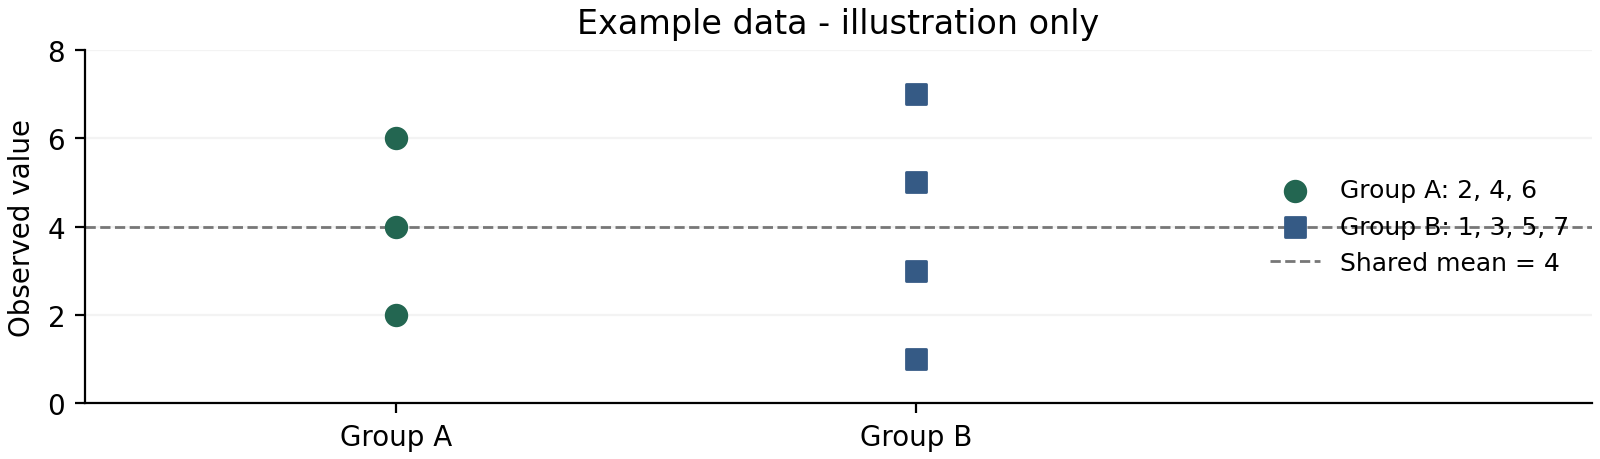
\includegraphics[width=0.9\linewidth]{figures/example-results.png}
  \caption{Example image: observations and means of illustrative data (replace with your own)}
  \label{fig:workflow}
\end{figure}

Figure~\ref{fig:workflow} is an example image included from a PNG file. Equal means do not imply
identical distributions; a full analysis should also report dispersion.
These data illustrate the template and are not empirical research findings.
\end{solution}
